\subsection{Final selection}
\label{sec:enujjFinalSelection}
   
Table~\ref{tab:enujjFinalSelection} shows the number of events
for the data, the backgrounds, and the LQ signal, after applying the final, optimized \enujj~selection 
criteria summarized in Table~\ref{tab:enujjOptimizedCuts}.
Figures~\ref{fig:st_mej_fullSelection400_enujj} and~\ref{fig:st_mej_fullSelection600_enujj} show the 
distributions of \st~and the selected electron-jet invariant mass, \mej, after the full selection 
optimized for \MLQ$=400$ and 600~\GeV, respectively. 
The dominant background contributions are from \ttbar~and \wjets~events, 
while the contribution from the other backgrounds is below \OtherBackgroundContributionINenujj~for 
the LQ masses within the current reach of this analysis. 
Good agreement is observed between the data and the background 
prediction, within uncertainties.    

\begin{table} 
  \small 
  \begin{tabular}{l | c | c | c | c | c | c | c} 
    $M_{LQ}$ & LQ Signal & W+Jets & $t\bar{t}$ & QCD & Other & Data &  Total BG \\ 
    \hline 
    \hline 
    Presel & -                     &  $ 20108 \pm 99  $ & $ 9301 \pm 42   $ & $ 3267 \pm 26 $     & $ 1913 \pm 53 $   &34135 & $ 34590 \pm 120 $ \\ 
    \hline 
    250    & $ 1703.5 \pm 13.8 $   &  $ 190  \pm 9.2  $ & $ 195  \pm 6.2  $ & $ 31.7  \pm 1.2  $  & $ 43.3 \pm 2.19 $ &456 & $ 460.4 \pm 11.4 $ \\ 
    350    & $ 285.54 \pm 2.06 $   &  $ 52.1 \pm 4.8  $ & $ 34.2 \pm 2.6  $ & $ 15.2  \pm 0.97 $  & $ 10.9 \pm 0.92 $ &89 & $ 112.4 \pm 5.6 $ \\ 
    400    & $ 126.01 \pm 0.82 $   &  $ 28.7 \pm 3.6  $ & $ 17.5 \pm 1.8  $ & $ 6.20  \pm 0.46 $  & $ 6.01 \pm 0.77 $ &43 & $ 58.4 \pm 4.1 $ \\ 
    450    & $ 68.38 \pm 0.43 $    &  $ 19.7 \pm 2.9  $ & $ 12.2 \pm 1.5  $ & $ 3.01  \pm 0.31 $  & $ 4.13 \pm 0.44 $ &30 & $ 39.1 \pm 3.3 $ \\ 
    500    & $ 34.70 \pm 0.23 $    &  $ 13.3 \pm 2.4  $ & $ 6.3  \pm 1.1  $ & $ 1.72  \pm 0.22 $  & $ 2.80 \pm 0.37 $ &20 & $ 24.2 \pm 2.6 $ \\ 
    550    & $ 16.25 \pm 0.10 $    &  $ 2.98 \pm 0.95 $ & $ 3.38 \pm 0.82 $ & $ 0.65  \pm 0.10 $  & $ 1.46 \pm 0.26 $ &9 & $ 8.5 \pm 1.3 $ \\ 
    600    & $ 9.442 \pm 0.056 $   &  $ 2.45 \pm 0.87 $ & $ 2.33 \pm 0.67 $ & $ 0.57  \pm 0.10 $  & $ 1.29 \pm 0.25 $ &7 & $ 6.6 \pm 1.1 $ \\ 
    650    & $ 5.202 \pm 0.032 $   &  $ 2.03 \pm 0.83 $ & $ 1.01 \pm 0.41 $ & $ 0.335 \pm 0.079 $ & $ 0.76 \pm 0.20 $ &5 & $ 4.14 \pm 0.95 $ \\ 
    750    & $ 1.851 \pm 0.010 $   &  $ 1.45 \pm 0.65 $ & $ 0.62 \pm 0.31 $ & $ 0.287 \pm 0.080 $ & $ 0.65 \pm 0.18 $ &5 & $ 3.01 \pm 0.75 $ \\ 
    850    & $ 0.6973 \pm 0.0037 $ &  $ 1.22 \pm 0.61 $ & $ 0.62 \pm 0.31 $ & $ 0.251 \pm 0.078 $ & $ 0.61 \pm 0.19 $ &5 & $ 2.70 \pm 0.71 $ \\ 
  \end{tabular}
  \caption{Number of events after the final \enujj~selection. Only statistical uncertainties are reported.}
  \label{tab:enujjFinalSelection}
\end{table}

\begin{figure}[htbp]
  \begin{center}
    \begin{tabular}{cc}
      \resizebox{7.5cm}{!}{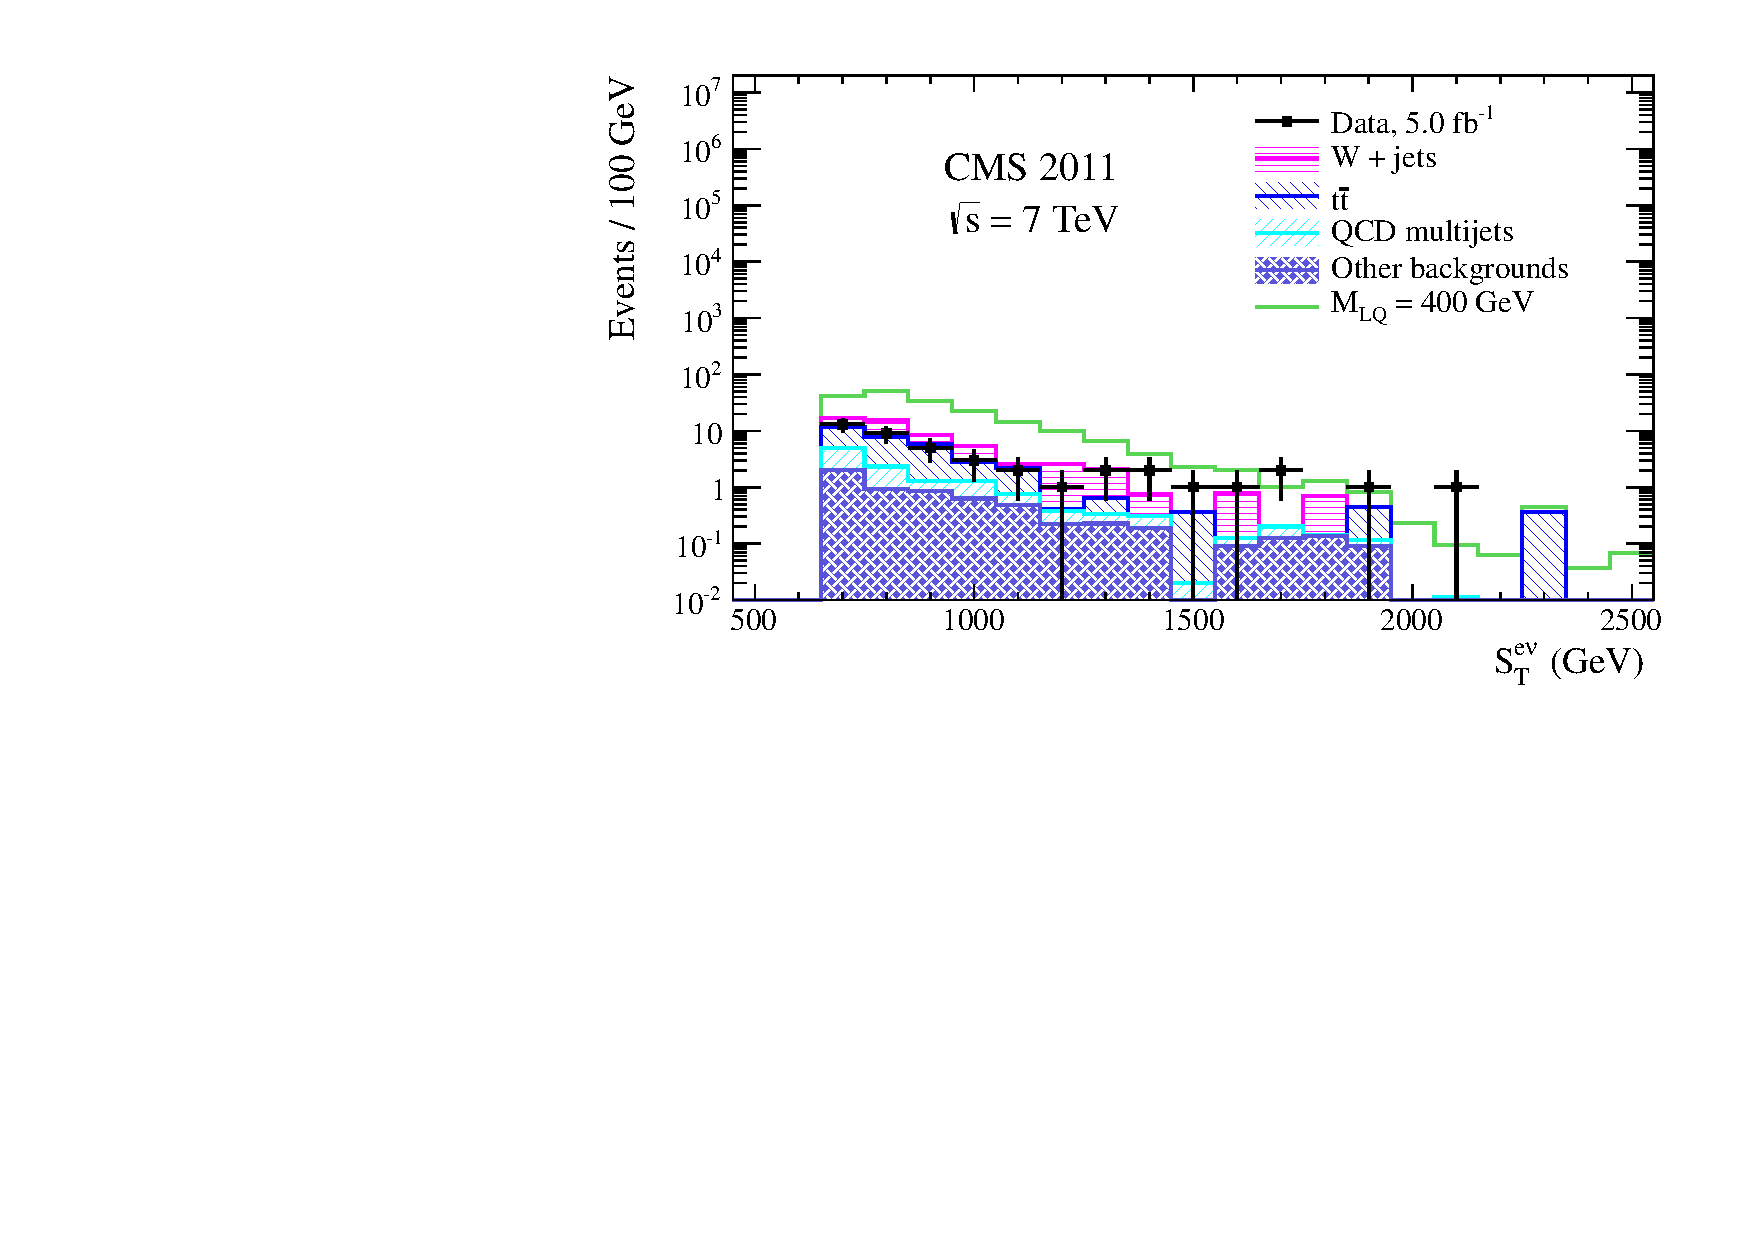
\includegraphics{tex/analysis/event_selection/fig/enu/final_selection/sT_LQ400_enujj_WZSherpa_MT120_OldRereco.pdf}} &
      \resizebox{7.5cm}{!}{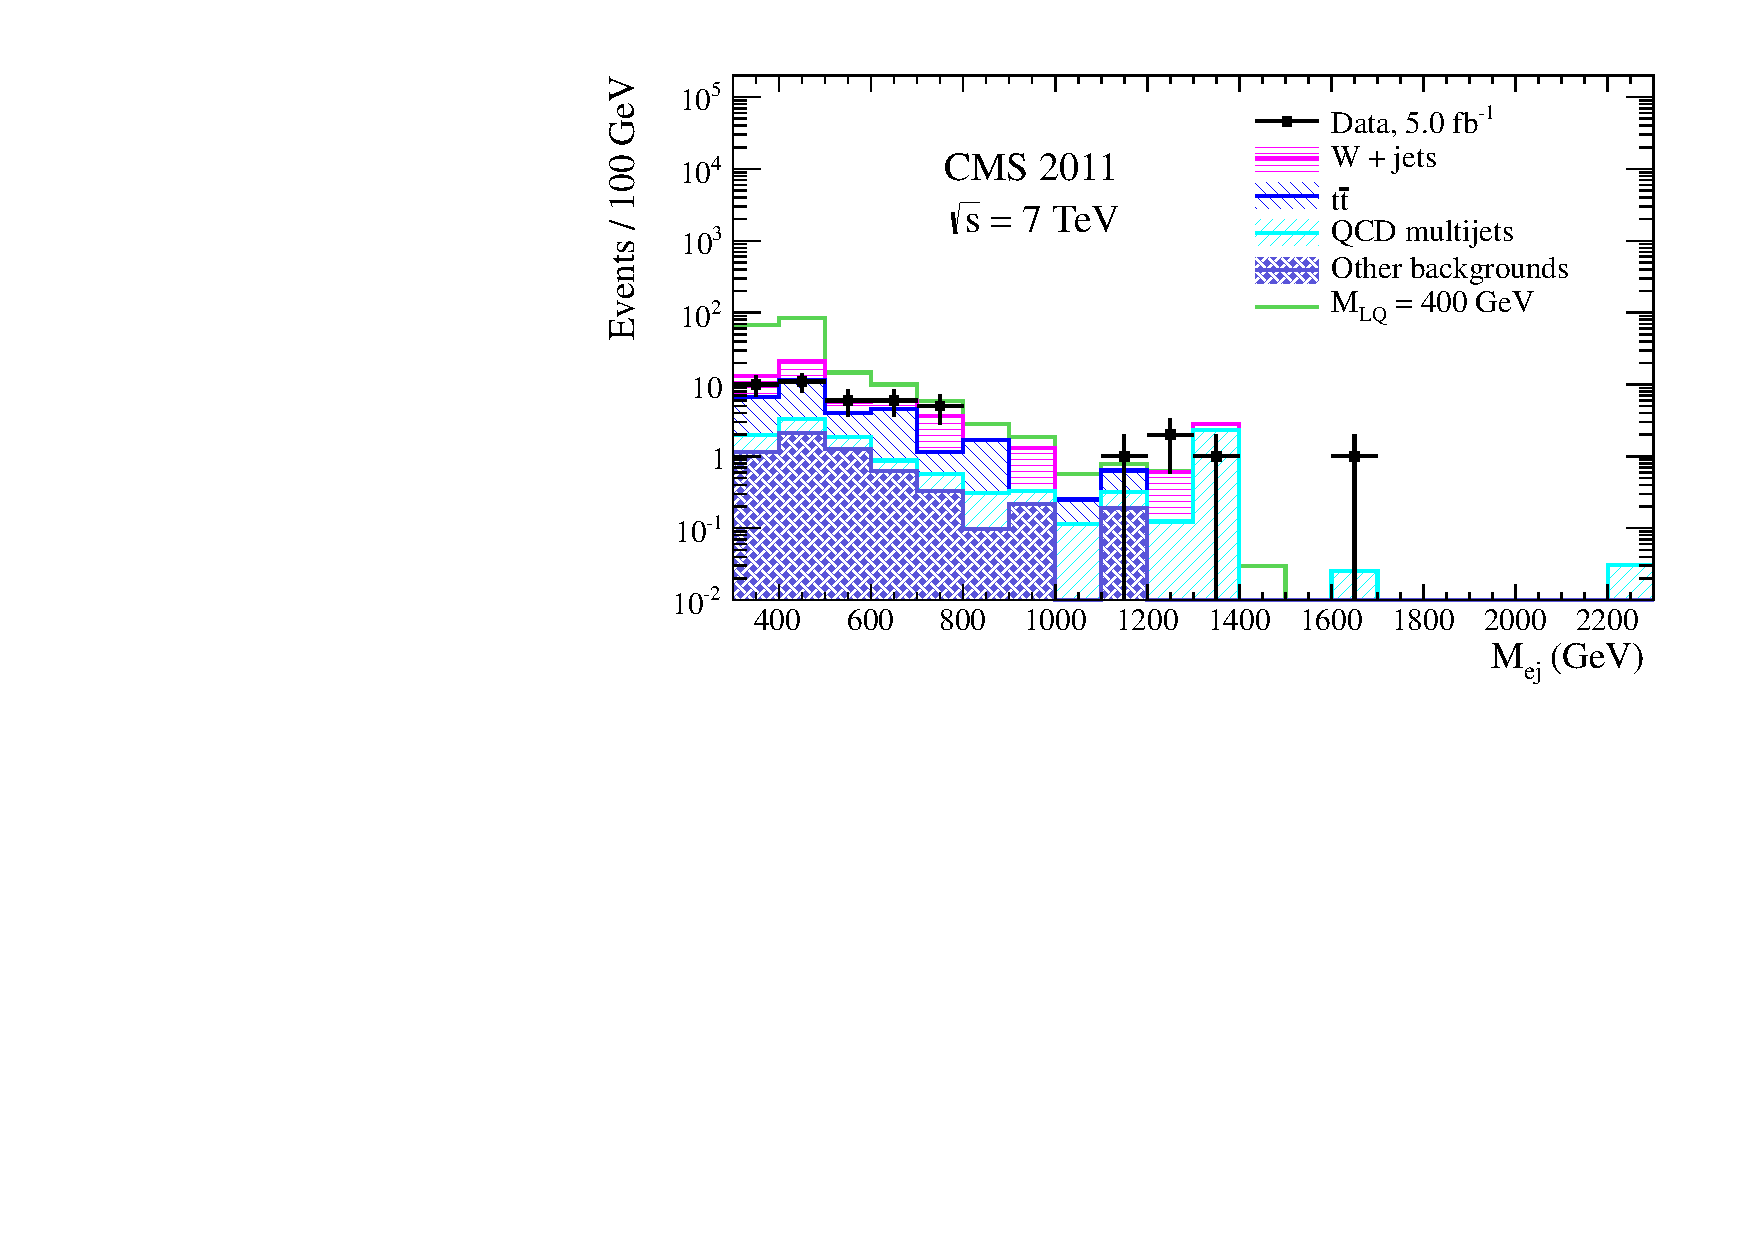
\includegraphics{tex/analysis/event_selection/fig/enu/final_selection/Mej_LQ400_enujj_WZSherpa_MT120_OldRereco.pdf}} \\
    \end{tabular}
    \caption{The \st (left)
             and \mej (right) distributions 
             for events passing the full \enujj selection optimized for \MLQ$=400$~\GeV.}
    \label{fig:st_mej_fullSelection400_enujj}
  \end{center}
\end{figure}

\begin{figure}[htbp]
  \begin{center}
    \begin{tabular}{cc}
      \resizebox{7.5cm}{!}{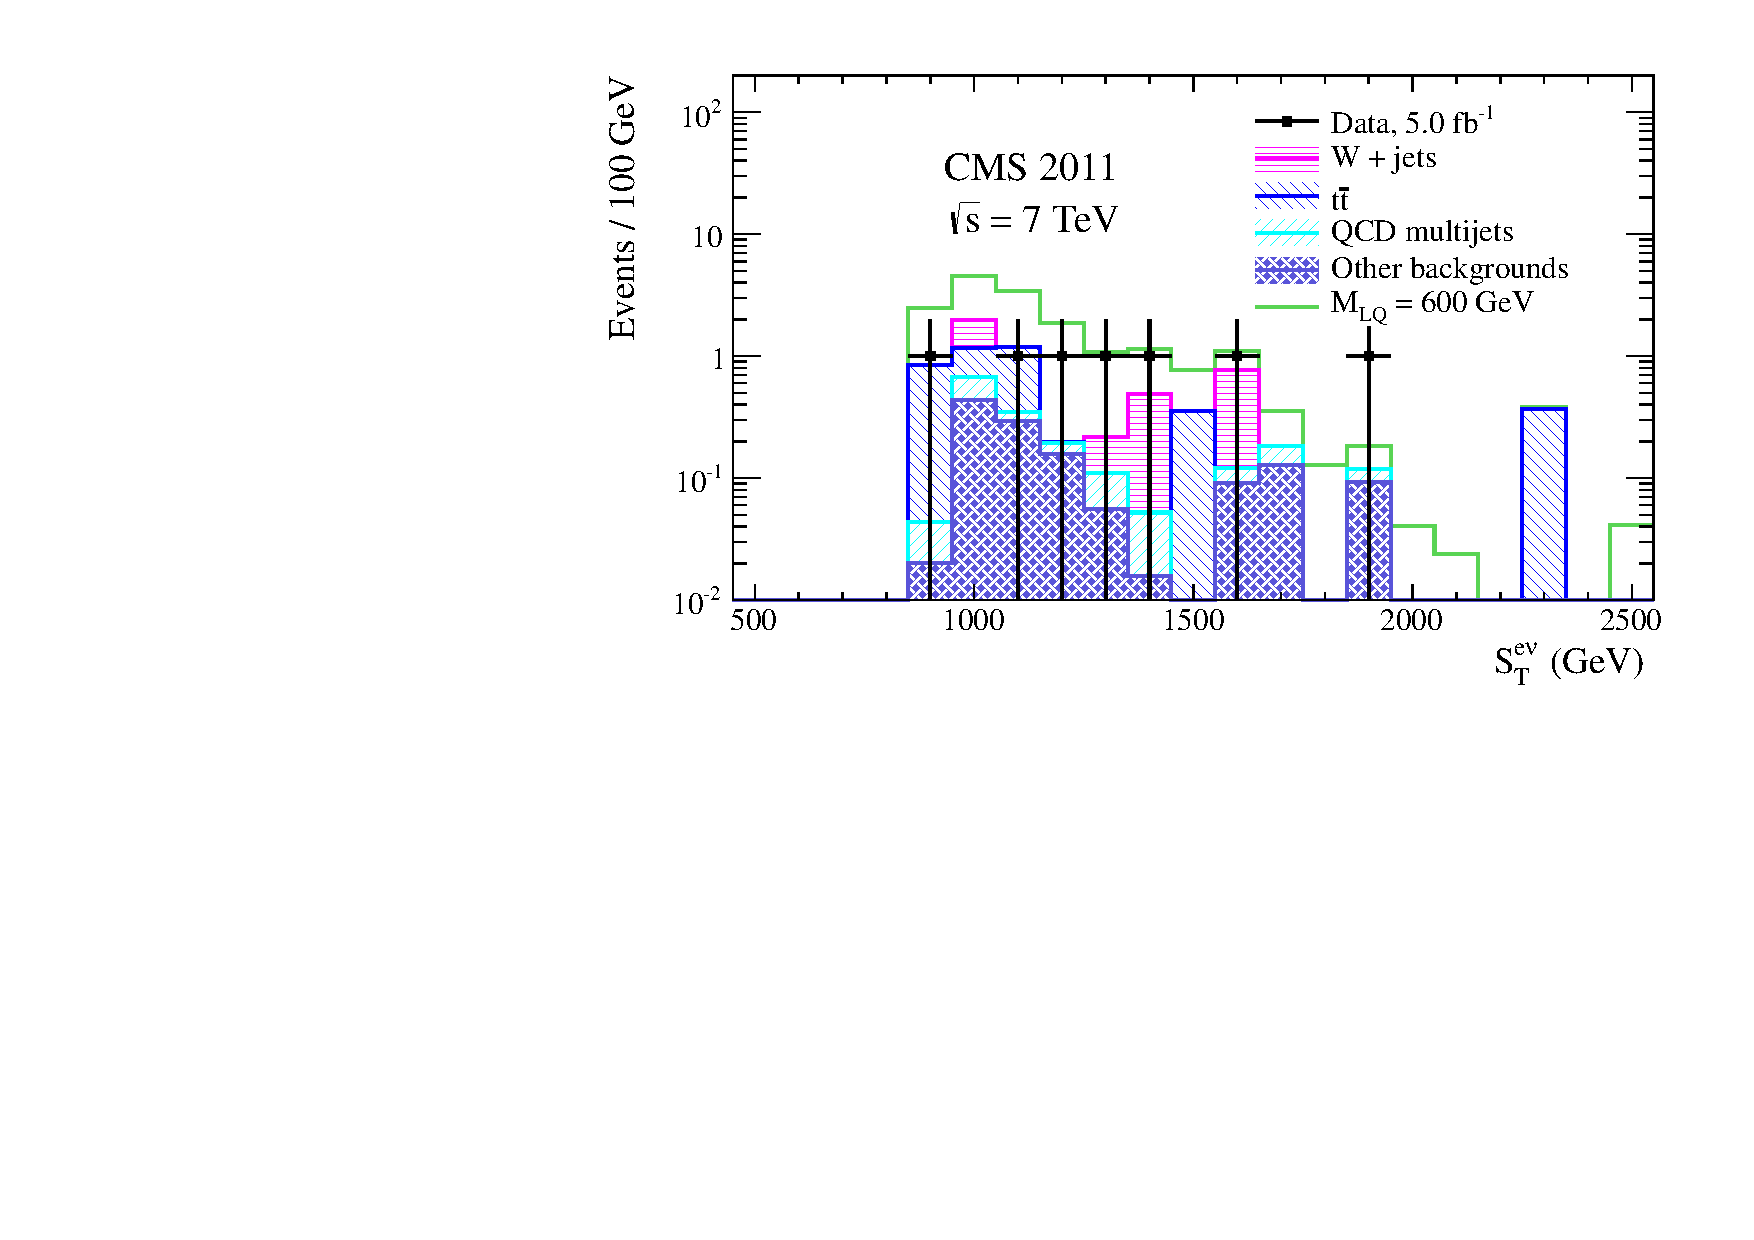
\includegraphics{tex/analysis/event_selection/fig/enu/final_selection/sT_LQ600_enujj_WZSherpa_MT120_OldRereco.pdf}} &
      \resizebox{7.5cm}{!}{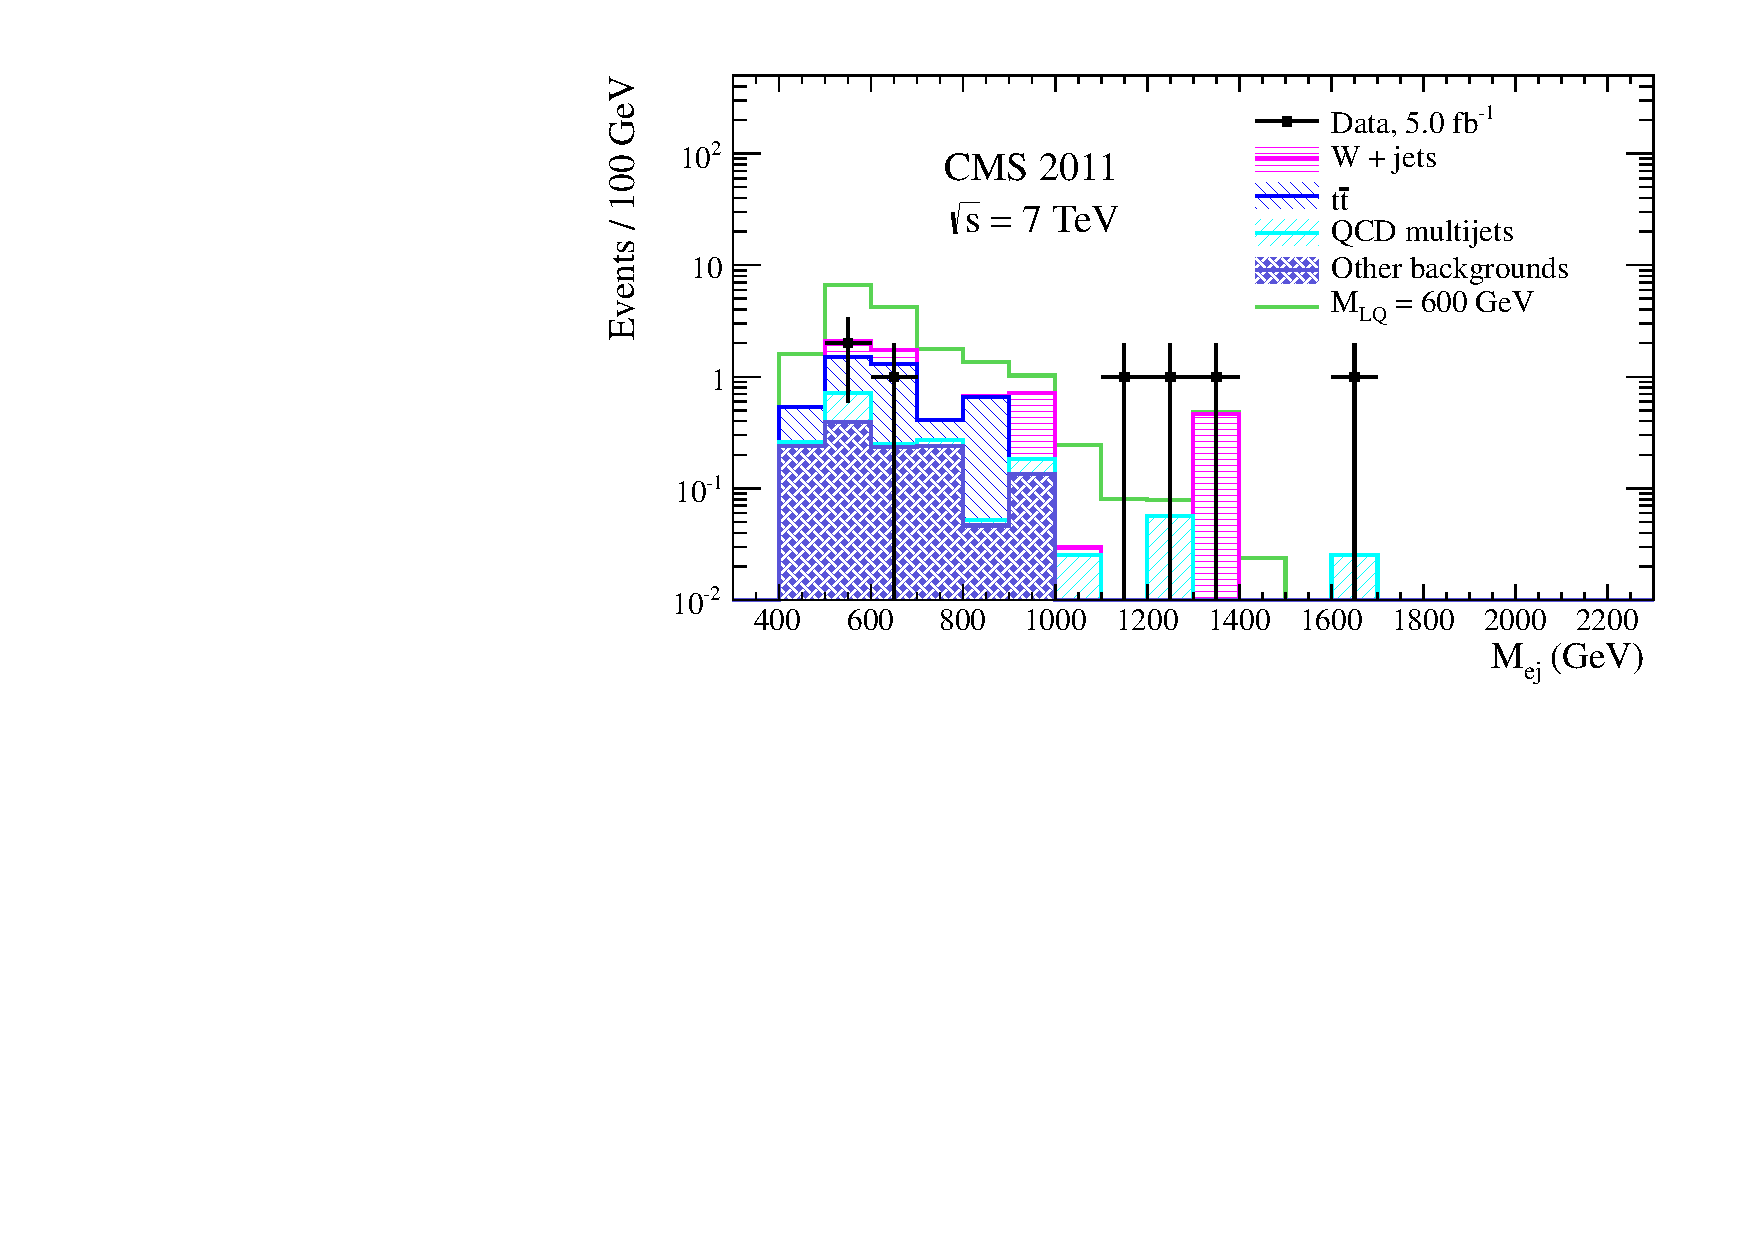
\includegraphics{tex/analysis/event_selection/fig/enu/final_selection/Mej_LQ600_enujj_WZSherpa_MT120_OldRereco.pdf}} \\
    \end{tabular}
    \caption{The \st (left)
             and \mej (right) distributions 
             for events passing the full \enujj selection optimized for \MLQ$=600$~\GeV.}
    \label{fig:st_mej_fullSelection600_enujj}
  \end{center}
\end{figure}

